\documentclass[11pt,a4paper]{article}
\usepackage[spanish]{babel}
\usepackage[utf8]{inputenc}
\usepackage{acl2015}
\usepackage{times}
\usepackage{url}
\usepackage{latexsym}
\usepackage{graphicx}
\usepackage{blindtext, subfig}
\usepackage{dblfloatfix}
\usepackage{color}
\usepackage{float}

\title{Resultados obtenidos en la práctica de Text Mining en Social Media.}

\author{Francisco José Pérez Carrasco \\
  {\tt frapecar@upvnet.upv.es} \\}

\date{}

\begin{document}
\maketitle
\begin{abstract}
  En esta memoria se describen los resultados obtenidos de la practica realizada en la asignatura Text Mining en Social Media. En ella se han propuesto dos casos de uso que nos permiten poner en practica las diferentes técnicas de analisis de textos estudiadas en la asignatura. 
  
En concreto en este trabajo se han desarrolado dos métodos de análisis que nos permiten analizar textos procedentes de la red social Twitter y clasificarlos por género o por nacionalidad del autor.
Para ello se ha partido de un set de tweets clasificados proporcionados por el profesor. Estos ficheros han sido analizados y procesados para generar un Dataset que nos permite alimentar los diferentes modelos utilizados en la comparativa de este trabajo.

Por otro lado se ha realizado un benchmark con diferentes bolsas de palabras generadas a partir del TopX de las palabras más utilizadas por los grupos a clasificar (género o nacionalidad). Y diferentes clasificadores. Los resultados se han plasmado en diferentes gráficas y tablas donde se puede apreciar los clasificadores que obtienen mejores resultados en función del dataset introducido.
Por último se ha incluido una sección de conclusiones y trabajo futuro donde se hace una pequeña autocrítica de los resultados obtenidos y que podríamos hacer para mejorar tanto la exactitud de los clasificadores como el performance de los algoritmos y funciones utilizadas. 

\end{abstract}

\section{Introducción}

A lo largo del master se han cursado diferentes asignaturas que tratan de abordar los problemas del procesado de grandes volúmenes de datos. En concreto en la asignatura de \textit{Text Mining} en social media, nos hemos centrado en el análisis de texto para la red social Twitter. El objetivo de la práctica consiste en aplicar diferentes técnicas que nos permitan analizar con mayor o menor eficacia un número determinado de textos para intentar descubrir diferentes características del autor. Aplicando una serie de análisis y métodos podemos estimar por ejemplo la edad, el sexo, la nacionalidad y hasta incluso detectar si el autor está escribiendo en su lengua nativa o se trata de una lengua secundaria.

Aunque esta tarea parezca algo simple o que no puede resultar de interes, en la actualidad resulta de gran importancia la identificación y creación de distintos perfiles en diferentes ramas como pueden ser el análisis forense, la seguridad y el marketing. Identificar el perfil lingüistico de un acosador y utilizarlo como evidencia, o enfocar diferentes campañas de venta dependiendo de análisis del blogs o revisiones de productos pueden ser algunos casos de uso del \textit{Author Profiling} mejorado gracias al \textit{Text Mining}.

\section{Dataset}

Para el desarrollo de la práctica se ha partido de dos sets de ficheros xml (un set para training y otro para test) que contienen (la mayoría de ellos) 100 tweets de un usuario anonimizado por un ID. Estos ficheros tienen como nombre el identificador del usuario. Por otro lado disponemos de un fichero (truth.txt) que contiene el identificador, el género y la nacionalidad del usuario. 

Una vez inspeccionados los ficheros se ha procedido a la generación de un dataset. Para ello se han seguido los siguientes pasos:
\begin{itemize}
	\item \textbf{Procesado de fichero truth.txt }
    
    Leemos el fichero y almacenamos en un diccionario el id, el género y la nacionalidad de cada uno de los usuarios.
    \item \textbf{Procesado de listado de adjetivos }
    
    Leemos un fichero que descargamos de internet con un gran listado de adjetivos que posteriormente utilizaremos para alimentar el dataset.
    
    \item \textbf{Procesado de ficheros XML }
    
    Leemos los ficheros xml y almacenamos en una lista el identificador del usuario (procedente del nombre del fichero) y cada uno de los tweets contenidos en el fichero.

\item \textbf{Creación de las bolsas de palabras }

En este paso procesamos la lista de tweets que hemos generado en el paso anterior y componemos dos bolsas de palabras con el top X de las palabras más utilizadas por género. En el caso de clasificación de nacionalidad generaríamos tantas bolsas de palabras como nacionalidades quisieramos clasificar. Para esta función hemos parametrizado el valor del top X para poder realizar un benchmark.

\item \textbf{Enriquecimiento del dataset }

Para obtener mejores resultados, se han generado variables adicionales al dataset, que consideramos podrían ser utilidad para la clasificación. 
En primer lugar hacemos un conteo de los adjetivos masculinos y femenimos que contiene cada tweet (tanto en singular como en plural).
Continuamos con el número medio de palabras por tweet de cada autor.
Añadimos el número medio de preposiciones usadas en cada tweet.
Y por último el número medio de emojis por tweet.

\end{itemize}

Como resultado final disponemos de un dataset con un número fijo de columnas (7) que corresponden con las variables generadas (id usuario, media de palabras, adjetivos masculinos, adjetivos femeninos, media de preposiciones, media de emojis, estimación de si es masculino o femenino en función de los adjetivos) y un número que varía en función de las bolsa de palabras generadas. 
Cabe destacar que añadimos a cada row del dataset tanto la bolsa de palabras masculina como la femenina.


\section{Propuesta del alumno}

Como se ha comentado en el apartado anterior, la propuesta plateada está basada en la creación de bolsas de palabras. Para ello se han definido una serie de funciones que nos proporcionan por un lado el top X de las palabras más utilizadas agrupadas por genero o nacionalidad (dependiendo del análisis a realizar) y por otro un contador de palabras que se encuentran en las bolsas generadas, que permite la definición de una matriz (numero de palabras por palabra y por tweet) para formar el dataset.

De forma adicional, se han definido funciones auxiliares que permiten el conteo de adjetivos masculinos, femeninos, número de preposiciones y emojis utilizados por tweet.

Con esto conseguimos generar un dataset que nos permite alimentar diferentes modelos de entrenamiento que permitan clasificar con el mínimo error posible, tanto el género como la nacionalidad de los autores de los tweets.

Para poder evaluar las diferentes combinaciones, se han propuesto por un lado, generar 4 datasets que incluyen las 7 variables generadas y las columnas del conteo obtenido las bolsas de 50, 100, 500 y 1000 palabras. Y por otro se han utilizado 4 clasificadores diferentes, que han sido entrenados con las 2/3 partes de los tweets que hemos leido del training y el tercio restante para la evaluación de los modelos como test.

\section{Resultados experimentales}

Para poder evaluar tanto los diferentes datasets propuestos como los clasificadores utilizados, se ha realizado una aplicación eh python que nos permite leer el dataset a evaluar y dividirlo en una parte para entrenamiento (2/3) y otra parte para test (1/3).

Además se han intoducido sondas de temporización que nos permiten medir el tiempo que necesitan los diferentes clasificadores para obtener la predicción y así poder evaluar tanto la exactitud como el performance de los mismos.

Para los experimentos realizados se ha utilizado la libreria sklearn de python y más concretamente los siguientes clasificadores:

\begin{itemize}
	\item \textbf{ Support Vector Machine }
    
    SVM configurado con un kernel lineal y los parámetros de penalización C = 1 y gamma = 1. Esta configuración se ha aplicado a los 4 datasets generados con las diferentes bolsas de palabras obteniendo unos tiempos de ejecución resumidos en la Tabla 1.
    
    \begin{table*}[h]
      \label{tabla_benchmark}
      \caption{Resultados del benchmark en los clasificadores.}
      \centering
      \begin{tabular}{p{0.17\linewidth}p{0.15\linewidth}p{0.15\linewidth}p{0.15\linewidth}p{0.15\linewidth}}
      \hline
       & t(s) Bolsa 50 & t(s) Bolsa 100 & t(s) Bolsa 500 & t(s) Bolsa 1000\\
      \hline
      SVM & 7.5 & 15.1 & 48.1 & 9.8 \\
      Decision Tree & 0.09 & 0.15 & 0.52 & 0.98 \\
      Random Forest & 0.25 & 0.25 & 0.23 & 0.26 \\
      Neural Network & 2.5 & 3.8 & 2.9 & 3.2 \\
      \hline
      \end{tabular}
    \end{table*}

	\item \textbf{ Decision Tree }
    
    El arbol de decisión ha sido configurado con los parámetros por defecto. Esta configuración se ha aplicado a los 4 datasets generados con las diferentes bolsas de palabras obteniendo unos tiempos de ejecución resumidos en la Tabla 1.
    
	\item \textbf{ Random Forest }
    
    Para el Random Forest se han utilizado los parámetros de configuración n-jobs = 2 y random-state = 0. Esta configuración se ha aplicado a los 4 datasets generados con las diferentes bolsas de palabras obteniendo unos tiempos de ejecución resumidos en la Tabla 1.

	\item \textbf{ Neural Networks }
    
    En la red neuronal se ha utilizado un clasificador Perceptron multicapa con una configuración de hidden-layer-sizes = (22,22,22) y un ma-iter = 500. Esta configuración se ha aplicado a los 4 datasets generados con las diferentes bolsas de palabras obteniendo unos tiempos de ejecución resumidos en la Tabla 1.    

\end{itemize}

Tras los tests realizados a los diferentes clasificadores con los datasets generados con las bolsas de 50, 100, 500 y 1000 palabras, en la Tabla 1 se puede observar que SVM en el dataset generado con la bolsa de 500 palabras tarda en realizar la clasificación un tiempo que sobrepasa en 1 orden de magnitud los tiempos de ejecucion para el resto de datasets, e incluso en 1 o 2 ordenes de magnitud el tiempo de ejecucion del resto de clasificadores. Esto puede ser debido a que este dataset genera alguna inestabilidad en el algoritmo SVM y le cuesta generar la predicción. 

Por otro lado también se puede observar como el arbol de decisión necesita más tiempo para obtener las predicciones al utilizar datasets con bolsas de palabras mayores. Sin embargo en el caso de Random Forest y las redes neuronales obtienen tiempos de ejecución similares para los diferentes datasets.

Con respecto al accuracy obtenido para las diferentes bolsas de palabra y los diferentes clasificadores se han realizado diferentes ejecuciones de de la aplicación desarrollada en python para generar tanto una comparativa gráfica que podemos observar en las Figuras \ref{A_50}, \ref{A_100}, \ref{A_500} y \ref{A_1000}.

\begin{figure}[H]
\centering
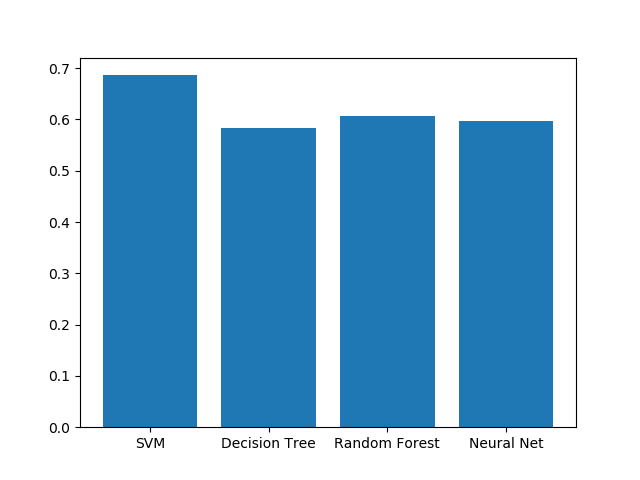
\includegraphics[width=0.21\textwidth]{.//50.png}
\caption{Accuracy del dataset 50.}
\label{A_50}
\end{figure}

\begin{figure}[H]
\centering
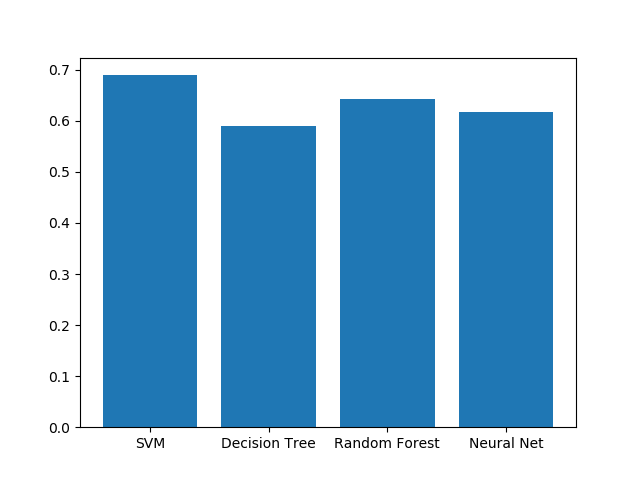
\includegraphics[width=0.21\textwidth]{.//100.png}
\caption{Accuracy del dataset 100.}
\label{A_100}
\end{figure}

\begin{figure}[H]
\centering
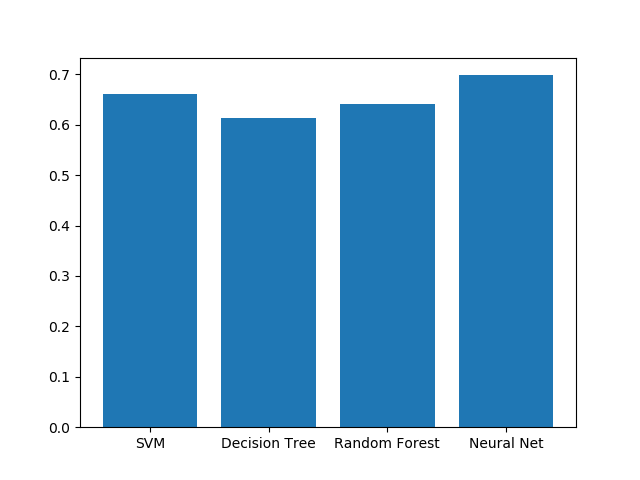
\includegraphics[width=0.21\textwidth]{.//500.png}
\caption{Accuracy del dataset 500.}
\label{A_500}
\end{figure}

\begin{figure}[H]
\centering
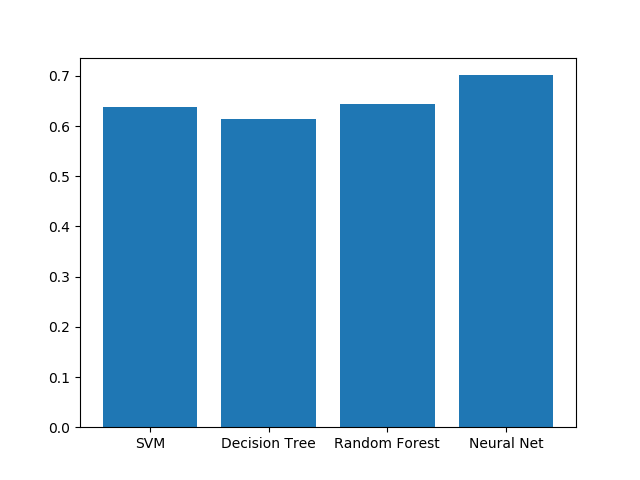
\includegraphics[width=0.21\textwidth]{.//1000.png}
\caption{Accuracy del dataset 1000.}
\label{A_1000}
\end{figure}

\begin{table*}[ht]
\caption{Porcentajes de acierto obtenidos.}
\label{accuracy}
\centering
\begin{tabular}{p{0.15\linewidth}p{0.15\linewidth}p{0.15\linewidth}p{0.15\linewidth}p{0.15\linewidth}p{0.15\linewidth}}
\hline
Nº Palabras & SVM & Decision Tree & Random Forest & Neural Net. & Tiempo (s)\\
\hline
50 & 0.68629 & 0.58244 & 0.60706 & 0.59743 & 9.17\\
100 & \textbf{0.68950} & 0.59207 & \textbf{0.64346} & 0.60278 & 17.77\\
500 & 0.66059 & 0.59100 & 0.64132 & 0.69486 & 52.68\\
1000 & 0.63811 & \textbf{0.59314} & 0.64346 & \textbf{\textcolor{red}{0.69700}} & 12.81\\
\hline
\end{tabular}
\end{table*}

La Tabla \ref{accuracy} resume los resultados obtenidos tras la ejecución de los diferentes clasificadores con los diferentes datasets. Como vemos, los mejores resultados se han obtenido para un clasificador basado en redes neuronales y un dataset generado a partir de una bolsa de 1000 palabras.

Sin embargo, obtenemos resultados similares en el clasificador basado en SVM con una precisión similar al basado en redes neuronales utilizando una bolsa de palabras inferior. Además se puede observar que dependiendo del clasificador utilizado, no por utilizar más variables se obtienen mejores resultados. En el caso del clasificador SVM, se obtiene un máximxo para 100 palabras y obtenemos resultados peores tanto en performance como en precisión si utilizamos bolsas de palabras mayores.

\section{Conclusiones y trabajo futuro}

Cómo conclusiones, podemos decir que la práctica nos ha permitido realizar el diseño de un analizador de \textit{Author Profiling} desde cero. 

Hemos conseguido procesar un set de ficheros con 100 tweets cada uno, y generar un dataset con una serie de variables calculadas a partir del estudio de los tweets y las diferentes técnicas estudiadas en clase (número total de palabras, adjetivos, preposiciones ...). Generar diferentes bolsas de palabras en función del topX que decidamos y añadirlas al dataset a procesar. 

Y por último hemos generado a partir del dataset un subgrupo de entrenamiento y otro de testing para evaluar los diferentes clasificadores elegidos para el desarrollo de la práctica.

Como conclusión general podemos decir que no por un mayor número de variables en el dataset obtenemos mejores resultados. Realizar un estudio de los datos a analizar y el problema planteado es una fase muy importante en este tipo de trabajos para generar variables de calidad que nos permitan obtener resultados de calidad.

Con respecto a los trabajos futuros, durante la práctica solo fuimos capaces de evaluar nuestros modelos para la detección de genero. Sería interesante generar las bolsas de palabras por paises e incluso tratar de generar bolsas con palabras que aparezcan en unos grupos y en otros no.

Otro trabajo a realizar sería aplicar los modelos diseñados a los ficheros de test, ya que solo hemos podido evaluar los tweets del set de training. Además sería interesante comprobar los resultados contra el \textit{baseline} proporcionado y evaluar si el trabajo realizado en esta practica es satisfactorio.

Para finalizar, como posibles mejoras en los algoritmos, en la parte de detectar la nacionalidad, sería interesante tratar de identificar por medio de expresiones regulares urls y extraer del dominio el país de procedencia. En la parte de detección de genero podríamos tratar de generar bolsas con por temas (deportes, tiendas, ropa ...), así podríamos identificar el genero por tematica. 

\begin{thebibliography}{}

\bibitem{authorProf} 
Author Profiling,
\\\texttt{https://pan.webis.de/clef18/pan18-
web/author-profiling.html}


\bibitem{MoadhGuefrech}
Moadh Guefrech.
\newblock 2015.
\newblock {\em Author profiling: Gender and Age detectionText Mining Project Report.}
\newblock Prentice-{Hall}.

\end{thebibliography}

\end{document}
